\section{System STLC-Impure}

This chapter describes an extension of system STLC-Pure, where there
exists both effect-disciplined functions (stoic functions) and
effect-arbitrary functions (libertine functions). As there's a
subtyping between the two kinds of functions, it's natural to
integrate subtyping in the system.

We'll first introduce the formalization, then discuss soundness and
effect safety. In the discussion, we'll focus on its difference from
system STLC-Pure.

\subsection{Definitions}

Initially, we arrived at a formualtion of the system shown in
Figure~\ref{fig:stlc-impure-definition-first}. It's a straight-forward
extension of SLTC-Pure with subtyping and libertine functions. Note
that in this formulation, we need to change the definition of the
\emph{pure} function to exclude libertine function types in the pure
environment. This restriction is important, because we're not sure
what side effects there might be inside libertine functions. If we
allow stoic functions have access to libertine functions, we'll loose
the ability to track the effects of stoic functions in the type
system.

The definition is all good, except that perservation breaks! The
problem is caused by using an impure term as \emph{Top}. To see a
concrete example, let's assume $\Gamma = \{c:E\}$. It's obvious that
following term is well-typed under $\Gamma$ as $B \to Top$:

\begin{center}
  $(\lambda x:Top. \; \lambda y:B. \; x) \; c$
\end{center}

However, after one evaluation step\footnote{Note that variables are
  values, thus we can take a step here. We can also construct a
  counter-example by wrap $c$ in a lambda abstraction like
  $\lambda x:B. c$.}, we get the term $\lambda y:B. \; c$, which can
at best be typed as $B \Rightarrow Top$. Thus preservation doesn't
hold in current formulation. This problem leads us to two different
formuations.

\begin{figure}
\begin{framed}

% multi-column separator
\setlength{\columnseprule}{0.4pt}
\begin{multicols}{2}

\textbf{Syntax}

\begin{tabu} to \linewidth {l l l X[r]}
  t   & ::= &                    & terms:               \\
      &     &  x                 & variable             \\
      &     & $\lambda$ x:T.t    & abstraction          \\
      &     & t t                & application          \\
\\
  v   & ::= &                    & values:              \\
      &     & $\lambda$ x:T.t    & abstraction value    \\
      &     & x                  & variable value       \\
\\
  T   & ::= &                    & types:               \\
      &     & \colorbox{shade}{Top}  & Top type             \\
      &     & B                  & basic type           \\
      &     & E                  & capability type      \\
      &     & T $\to$ T          & type of stoics       \\
      &     & \colorbox{shade}{T $\Rightarrow$ T} & type of libertines   \\
\end{tabu}

\hfill\\

\textbf{Evaluation} \hfill \framebox[1.2\width][r]{$t \longrightarrow t'$}

\infrule[E-App1]
{ t_1 \longrightarrow t'_1 }
{ t_1 \; t_2 \longrightarrow t'_1 \; t_2 }

\infrule[E-App2]
{ t_2 \longrightarrow t'_2 }
{ v_1 \; t_2 \longrightarrow v_1 \; t'_2 }

\infax[E-AppAbs]
{ (\lambda x:T.t_1) v_2 \longrightarrow [x \mapsto v_2]t_1 }

\textbf{Pure Environment}

\begin{center}
\begin{tabular}{l c l}
pure($\varnothing$)                   & = &   $\varnothing$ \\
pure($\Gamma$, x: E)                  & = &  pure($\Gamma$) \\
\rowcolor{gray!40}
pure($\Gamma$, x: S $\Rightarrow$ T)  & = &  pure($\Gamma$) \\
pure($\Gamma$, x: T)                  & = &  pure($\Gamma$), x: T     \\
\end{tabular}
\end{center}

\columnbreak

\textbf{Typing}  \hfill \framebox[1.2\width][r]{$\Gamma \vdash x : T$}

\infrule[T-Var]
{ x: T \in \Gamma }
{ \Gamma \vdash x : T }

\infrule[T-Abs1]
{ pure(\Gamma),\; x: S \vdash t_2 : T }
{ \Gamma \vdash \lambda x:S.t_2 : S \to T }

\infrule[T-Abs2]
{  \colorbox{shade}{$\Gamma,\; x: S \vdash t_2 : T$} }
{  \colorbox{shade}{$\Gamma \vdash \lambda x:S.t_2 : S \Rightarrow T$} }

\infrule[T-App]
{ \Gamma \vdash t_1 : S \to T \andalso \Gamma \vdash t_2 : S }
{ \Gamma \vdash t_1 \; t_2 : T }

\infrule[T-Sub]
{  \colorbox{shade}{$\Gamma \vdash t : S \andalso S <: T$} }
{  \colorbox{shade}{$\Gamma \vdash t : T$} }

\colorbox{shade}{\textbf{Subtyping}}  \hfill \framebox[1.2\width][r]{$S <: T$}

\infax[S-Top]{ T <: Top }

\infax[S-Refl]{ T <: T }

\infrule[S-Trans]
{ S <: U \andalso U <: T }
{ S <: T }

\infrule[S-Degen]
{ S \to T }
{ S \Rightarrow T }

\infrule[S-Fun1]
{ S1 <: S2 \andalso T2 <: T1 }
{ S2 \to T2 <: S1 \to T1 }

\infrule[S-Fun2]
{ S1 <: S2 \andalso T2 <: T1 }
{ S2 \Rightarrow T2 <: S1 \Rightarrow T1 }

\hfill\\

\end{multicols}
\end{framed}

\caption{System STLC-Impure First Formulation}
\label{fig:stlc-impure-definition-first}
\end{figure}

The first one is to introduce two different Top types, one is pure and
the other is impure. The capability type E and libertine function type
$S \Rightarrow T$ are not sutype of the pure Top. The subtyping
hierarchy is shown in Figure~\ref{fig:stlc-impure-subtyping-tree}. This
formulation works well, and we've proved soundness and effect safety
for the formulation. However, we lose the simplicity in the type
system. And it's counter-intuitive to forbid Top in pure environments,
as we cannot create side effects with a variable of type Top.

\begin{figure}
\centering

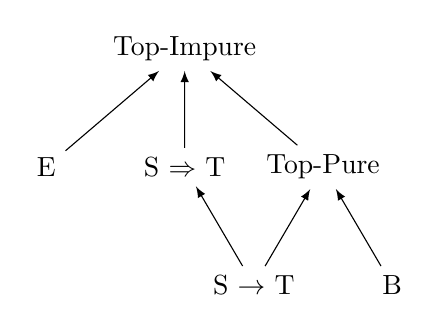
\begin{tikzpicture}[sibling distance=5em,
  every node/.style = {align=center},
  edge from parent/.style={draw,latex-}]
  \node {Top-Impure}
  child { node {E} }
  child { node (libertine) {S $\Rightarrow$ T} }
  child { node {Top-Pure}
    child { node (stoic) {S $\to$ T} }
    child { node {B} } };
  \path [draw, -latex] (stoic) -- (libertine);
\end{tikzpicture}

\caption{Subtyping: Top-Pure and Top-Impure}
\label{fig:stlc-impure-subtyping-tree}
\end{figure}

The second possibility is to keep the elegance of the type system and
changes the evaluation rules. We know that all terms of the type Top
are equivalent, because we can do nothing with a term of type Top. It
implies we can substitute them arbitrarily without changing the
meaning of the term. This observation inspires us to introduce a
\emph{top} value and change the standard E-AppAbs rule to two
evaluation rules as follows:

\infrule[E-AppAbs1]
{ T \neq Top }
{ (\lambda x:T.t_1) v_2 \longrightarrow [x \mapsto v_2]t_1 }

\infrule[E-AppAbs2]
{ T = Top }
{ (\lambda x:T.t_1) v_2 \longrightarrow [x \mapsto top]t_1 }

The two rules have the effect that if a function takes a parameter of
type Top, then when called it will drop the parameter and replace it
with the \emph{top} value. We follow this approach in the formulation
and the full definition is presented in
Figure~\ref{fig:stlc-impure-definition}.

\begin{figure}
\begin{framed}

% multi-column separator
\setlength{\columnseprule}{0.4pt}
\begin{multicols}{2}

\textbf{Syntax}

\begin{tabu} to \linewidth {l l l X[r]}
  t   & ::= &                    & terms:               \\
      &     & \colorbox{shade}{top} & top value            \\
      &     & x                  & variable             \\
      &     & $\lambda$ x:T.t    & abstraction          \\
      &     & t t                & application          \\
\\
  v   & ::= &                    & values:              \\
      &     & $\lambda$ x:T.t    & abstraction value    \\
      &     & x                  & variable value       \\
      &     & \colorbox{shade}{top}  & top value            \\
\\
  T   & ::= &                    & types:               \\
      &     & \colorbox{shade}{Top}  & Top type             \\
      &     & B                  & basic type           \\
      &     & E                  & capability type      \\
      &     & T $\to$ T          & type of stoics       \\
      &     & \colorbox{shade}{T $\Rightarrow$ T} & type of libertines   \\
\end{tabu}

% \hfill\\
\vspace{0.1em}

\textbf{Evaluation} \hfill \framebox[1.2\width][r]{$t \longrightarrow t'$}

\infrule[E-App1]
{ t_1 \longrightarrow t'_1 }
{ t_1 \; t_2 \longrightarrow t'_1 \; t_2 }

\infrule[E-App2]
{ t_2 \longrightarrow t'_2 }
{ v_1 \; t_2 \longrightarrow v_1 \; t'_2 }

\infrule[E-AppAbs1]
{ \colorbox{shade}{$T \neq Top$} }
{ \colorbox{shade}{$(\lambda x:T.t_1) \; v_2 \longrightarrow [x \mapsto v_2]t_1$} }

\infrule[E-AppAbs2]
{ \colorbox{shade}{$T = Top$} }
{ \colorbox{shade}{$(\lambda x:T.t_1) \; v_2 \longrightarrow [x \mapsto top]t_1$} }

\textbf{Pure Environment}

\begin{center}
\begin{tabular}{l c l}
pure($\varnothing$)                   & = &   $\varnothing$ \\
pure($\Gamma$, x: E)                  & = &  pure($\Gamma$) \\
\rowcolor{gray!40}
pure($\Gamma$, x: S $\Rightarrow$ T)  & = &  pure($\Gamma$) \\
pure($\Gamma$, x: T)                  & = &  pure($\Gamma$), x: T     \\
\end{tabular}
\end{center}

\columnbreak

\textbf{Typing}  \hfill \framebox[1.2\width][r]{$\Gamma \vdash x : T$}

\infax[T-Top]{ \colorbox{shade}{$\Gamma \vdash top : Top$} }

\infrule[T-Var]
{ x: T \in \Gamma }
{ \Gamma \vdash x : T }

\infrule[T-Abs1]
{ pure(\Gamma),\; x: S \vdash t_2 : T }
{ \Gamma \vdash \lambda x:S.t_2 : S \to T }

\infrule[T-Abs2]
{  \colorbox{shade}{$\Gamma,\; x: S \vdash t_2 : T$} }
{  \colorbox{shade}{$\Gamma \vdash \lambda x:S.t_2 : S \Rightarrow T$} }

\infrule[T-App]
{ \Gamma \vdash t_1 : S \to T \andalso \Gamma \vdash t_2 : S }
{ \Gamma \vdash t_1 \; t_2 : T }

\infrule[T-Sub]
{  \colorbox{shade}{$\Gamma \vdash t : S \andalso S <: T$} }
{  \colorbox{shade}{$\Gamma \vdash t : T$} }

\colorbox{shade}{\textbf{Subtyping}}  \hfill \framebox[1.2\width][r]{$S <: T$}

\infax[S-Top]{ T <: Top }

\infax[S-Refl]{ T <: T }

\infrule[S-Trans]
{ S <: U \andalso U <: T }
{ S <: T }

\infrule[S-Degen]
{ S \to T }
{ S \Rightarrow T }

\infrule[S-Fun1]
{ S1 <: S2 \andalso T2 <: T1 }
{ S2 \to T2 <: S1 \to T1 }

\infrule[S-Fun2]
{ S1 <: S2 \andalso T2 <: T1 }
{ S2 \Rightarrow T2 <: S1 \Rightarrow T1 }

\hfill\\

\end{multicols}
\end{framed}

\caption{System STLC-Impure}
\label{fig:stlc-impure-definition}
\end{figure}

\subsection{Soundness}

We proved both progress and preservation in Coq based on the
locally-nameless representation.

\begin{theorem}[Progress]
If $\varnothing \vdash t : T$, then either $t$ is a value or there is some
$t'$ with $t \longrightarrow t'$.
\end{theorem}

\begin{theorem}[Preservation]
If $\Gamma \vdash t : T$, and $t \longrightarrow t'$, then $\Gamma
\vdash t' : T$.
\end{theorem}

As you can imagine, now we need to different substitution lemmas in
the proof of perservation, corresponding to the two reduction rules.

\begin{lemma}[Subsitution-Non-Top]
  If $\Gamma,\; x:S \vdash t : T$, s is a value, $S \neq Top$ and
  $\Gamma \vdash s : S$, then $\Gamma \vdash [x \mapsto s]t : T$.
\end{lemma}

\begin{lemma}[Subsitution-Top]
  If $\Gamma,\; x:Top \vdash t : T$, then $\Gamma \vdash [x \mapsto top]t : T$.
\end{lemma}

\subsection{Effect Safety}

\subsubsection{Definition}

\subsubsection{Proof}
